\chapter{Fundamentação teórica} \label{cap:teoria}
  
Neste capítulo será feita uma breve revisão das características principais das series temporais,  assim como das redes neurais, especialmente das que serão aplicadas no problema de interesse, chamadas de redes Multilayer Perceptron (MLP) e redes Gated Recurrent Unit (GRU).  

    \section{Métodos de Previsão de Demanda} 
    
        A previsão de demanda pode ser definida como um processo de busca de informações que geram vendas de um produto ou um conjunto de produtos.
        
        Em \citeonline{moreira1998} são definidos os métodos de previsão de demanda como processos que utilizam tais informações para estimar uma demanda futura, podendo se encaixar nesta definição desde métodos subjetivos e intuitivos até métodos matemáticos e computacionais. No mesmo trabalho, são classificado os modelos de previsão em dois grandes grupos: métodos qualitativos e métodos quantitativos.
        
         Em  \citeonline{Junior2007} foi feito a avaliação de  diversos métodos de previsão de demanda, os quais são esquematizados na Figura \ref{fig: metodosPrevisaoDemanda}. 
        
                  \begin{figure}[ht]
                  	\center{
                  	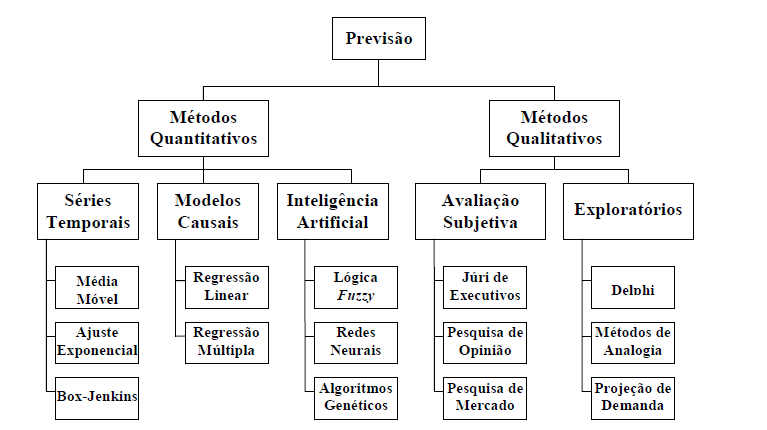
\includegraphics[width=\textwidth]{./Figs/01-junior-metodos-previsao-demanda.png}
                  	\caption{Métodos de previsão de demanda.}\caption*{  Fonte: \cite{Junior2007}.}
                  	\label{fig: metodosPrevisaoDemanda}}
                  \end{figure}
        
        Os métodos qualitativos são definidos em \cite{Junior2007} como um julgamento dos dados expostos sem processamento analítico, tais como agrupamento e classificação de dados. Esses métodos não fornecem novas informações numéricas nem  modelos preditivos.
        
        Já os métodos quantitativos são definidos, no mesmo trabalho, como sendo analíticos e baseados em  modelos matemáticos para realizar previsões. Esses métodos analisam padrões de comportamento de um histórico de dados, visando predizer comportamento futuro.
         
        Em \citeonline{Junior2007} também é mencionado que os dados coletados para modelos de previsão, ao ser projetados graficamente, evidenciam comportamentos que podem ser generalizados de forma subjetiva pelos gestores dos dados. Em todos os casos, a análise de dados é necessária para selecionar parâmetros de demanda objetivos para fazer predições. Porém, apenas a análise dos dados pode ser insuficiente,  e se realizada com critérios incorretos pode comprometer as conclusões dos estudos. 
        
        A análise de dados é um processo amplo que visa tratar os dados desde sua aquisição e pré-processamento até a sua interpretação a partir de ferramentas complexas de mineração. Nas diferentes etapas, são abrangidas diversas técnicas matemáticas, probabilísticas, estatísticas, computacionais e heurísticas.  Na Seção \ref{sec: timeseries} serão comentadas as principais características das séries temporais, o qual será o método de previsão aplicado ao problema prático de interesse. 
    
        \subsection{Séries Temporais} \label{sec: timeseries} 
         
            De acordo com  \citeonline{Morettin1987}, uma série temporal é um conjunto de observações ordenadas em função do tempo, comumente iguais, apresentando uma dependência serial entre ela. Também pode ser definida como uma realização de um conjunto de variáveis aleatórias $ X=\{x_1, x_2, \dots, x_T\}$, ordenadas no tempo, onde  $T$ representa o comprimento da série, como é feito em \cite{defts}. A relação entre as variáveis é comumente descrita pela função de distribuição conjunta delas, ou, em outros casos, pela media e covarianças. 
            
            Entre os objetivos do análise de séries temporais, podem ser destacados os seguintes: i) descrever o comportamento das séries identificando tendências e variações, ii) analisar e modelar  a dependência entre as observações, e iii) fazer previsões de valores futuros da série. 
            
            As series temporais tem uma componente determinística e uma componente aleatória, e podem ser contínuas ou discretas, dependendo do tipo de observação das variáveis. São chamadas de estacionárias quando as propriedades de média, variança e covariança são mantidas no tempo. A tendência faz referência à taxa de crescimento ou de decréscimo, podendo ser linear, exponencial ou amortecido. Já a oscilação da tendência é conhecida como ciclo. Além disso, podem apresentar sazonalidade, isto é, exibir comportamento que tende a se repetir em certo numero de períodos de tempo.
    
            Exemplos de cada uma dessas propriedades, assim como técnicas aplicadas para estudo e correção de cada uma delas podem ser vistas em \cite{tecnicas1}. Essas características, junto com o estudo da componente aleatória, fornecem informações de interesse para as aplicações práticas.  
            %\TODOR{Passar pra metodologia ou literatura, não falar do trabalho aqui}
            Devido ao objetivo deste trabalho, serão aplicadas series temporais para eventos com sazonalidade, a fim de estimar previsões. As técnicas para fazer isto usam métodos de regressão,  e algumas aplicações praticas podem ser vistas incluem  previsão de consumo de energia elétrica realizados , como feito em  \citeonline{Almeida2013}, \citeonline{RUAS2012} e \citeonline{Silva2010}, e da previsão de demanda de produtos cosméticos, como pode ser visto em \citeonline{Junior2007}.
    
    \section{Redes Neurais Artificiais}
    
        As redes neurais artificiais são ferramentas com raiz multidisciplinar, pois são nutridas por conhecimentos de neurociência, matemática, estatística, física, ciência da computação e engenharia \cite{Haykin1994}, e fazem parte da grande área de conhecimento denominada Inteligência Artificial (IA), termo cunhado em \cite{kaplan2019siri}.
        
        De forma resumida, poderia ser definido que "a inteligência artificial é o ramo da ciência da computação que se ocupa do comportamento inteligente." \cite{Luger2004}. Os sistemas de inteligência artificial buscam resolver funções e problemas inspirados em duas características humanas: capacidade de abstração e aprendizagem com o erro. 
        
        No contexto de IA um neurônio é uma unidade considerada fundamental para o processamento de informação, e as redes neurais são conjuntos de neurônios artificiais interconectados através de relações, funções lógicas e matemáticas \cite{Haykin1994}. Os neurônios de uma rede são capazes de processar múltiplos valores de entradas e reagir rapidamente produzindo uma resposta relacionada à essas entradas, simulando o comportamento do cérebro humano. 
        
        Inspirado por uma busca de um modelo computacional do neurônio biológico, o primeiro modelo de neurônio artificial, denominado MCP, foi proposto no artigo \textit{ A Logical Calculus of the Ideas Immanent in Nervous Activity.} \cite{mcculloch43a}, uma ilustração adaptada por \cite{lemos} deste modelo pode ser visualizada na figura \ref{fig: NeuronioArtificial}.
        
        McCuloch era psiquiatra e neuroanatomista e passou cerca de 20 anos refletindo e estudando sobre a representação do sistema nervoso, em 1942 ele convidou Pitts, que era matemático, para fazer parte das suas pesquisas.
        
        A estrutura do neurônio artificial reage a um vetor de entradas e as sinapses são representas por pesos numéricos. Uma função de transferência, também chamada função de ativação, avalia uma combinação linear dos valores da entrada e os pesos das sinapses, determinando se o neurônio é ativado ou não dependendo do valor obtido. Se o neurônio é ativado é emitido um valor de saída 1, caso contrário se emite um valor de saída 0.
            \begin{figure}[ht]
                \center{
                  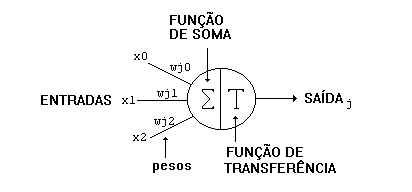
\includegraphics[width=0.65\textwidth]
                  {./Figs/02-neuronio-artificial.png}
                \caption{Neuronio Artificial. }\caption*{  Fonte:\cite{lemos}} \label{fig: NeuronioArtificial} }
            \end{figure}
            
        Todo o funcionamento deste modelo então é reduzido a responder se a soma ponderada recebida é maior que um valor numérico estabelecido. Contudo, associado a este neurônio não foi proposto uma forma automática para ajuste dos pesos, ou seja, não foi dado um algoritmo de aprendizagem para treinar o neurônio. Esse problema foi contornado posteriormente, pela formulação do Perceptron.
        
        Em \citeonline{Haykin1994} no capítulo 1.9 denominado \textit{Notas Históricas}, é apresentada com mais detalhes a fascinante história de desenvolvimento das redes neurais desde a concepção inicial do estudos do neurônio biológico até redes complexas de aprendizagem supervisionada chamadas de \textit{Máquinas de Vetor Suporte}.
            
        \subsection{Perceptron} \label{sec: perceptron}
    
            O modelo de neurônio proposto em \citeonline{mcculloch43a}, apesar de simular um neurônio biológico e resolver algumas tarefas lógicas e matemáticas, não atendia o objetivo principal da Inteligência Artificial: A capacidade de aprendizado. Para poder utilizar esta estrutura, era necessário conhecer o ajuste dos pesos das entradas, o qual não era um problema trivial em muitos casos. 
                        
            O primeiro neurônio com um algoritmo de aprendizado foi proposto em \citeonline{perceptron} e foi nomeado de Perceptron. Nesse trabalho, os pesos das conexões são ajustados de forma autônoma com a introdução de pesos associados e um valor bias, a fim de buscar um reconhecimento autônomo de padrões. Na Figura \ref{fig: perceptron} é apresentado um esquema do funcionamento da estrutura.
            
            \begin{figure}[ht]
            	\center{
              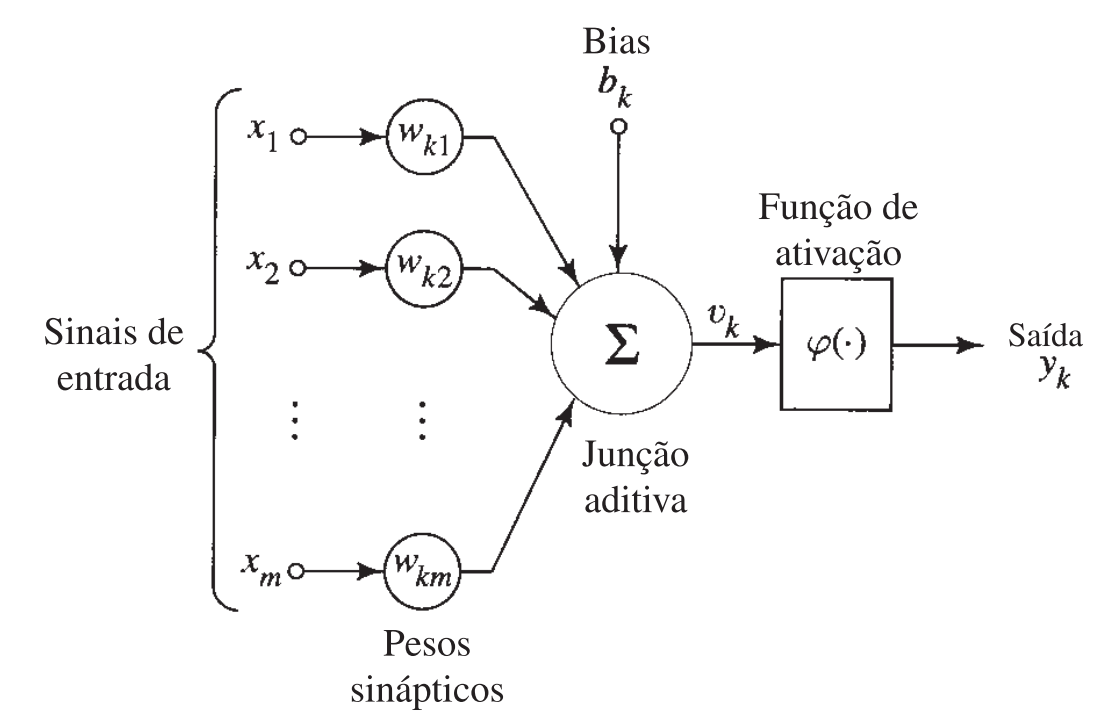
\includegraphics[width=0.65\textwidth]
              {./Figs/03-perceptron.png}
            \caption{Neurônio Artificial Perceptron. }\caption*{  Fonte: \citeonline{Haykin1994}} \label{fig: perceptron} }
            \end{figure}
            
            Porém, em \citeonline{perceptrons2} foi provado que, devido ao modelo aprendizado limitado a uma combinação linear, o perceptron poderia resolver apenas problemas linearmente separáveis. Na Figura \ref{fig:problemasLineares} são apresentados dois problemas simples, um que o perceptron pode resolver \textit{(a)}, e outro que não \textit{(b)}.
            
            \begin{figure}[ht]
              	\center{
              	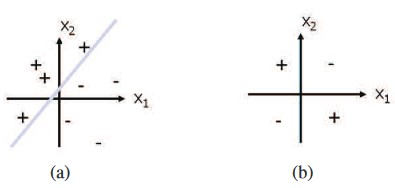
\includegraphics[width=0.8\textwidth]{./Figs/04-limite-perceptron.jpg}
              	\caption{Problema linearmente separável (a) e não separável (b).}\caption*{  Fonte:\cite{Flavia2014}.}
              	\label{fig:problemasLineares}
              	}	
            \end{figure}
            
            Quase duas décadas depois, foi apresentado em \cite{rede1} o primeiro modelo de rede neural, chamada de rede perceptron, aplicando o treinamento por combinações lineares à um conjunto de perceptrons interligados. Essa abordagem permitia resolver problemas mais complexos por meio de uma combinação de soluções. 
              
            A rede possuía apenas uma camada de entrada, uma única saída, e uma função de ativação  $ \varphi $ \cite{Haykin1994}. A função de ativação da rede perceptron ainda poderia ser linear ou não linear. Na Figura \ref{fig:activation_functions} são ilustradas algumas funções de ativação comumente utilizadas. 
            
             \begin{figure}[ht]
                \center{
            	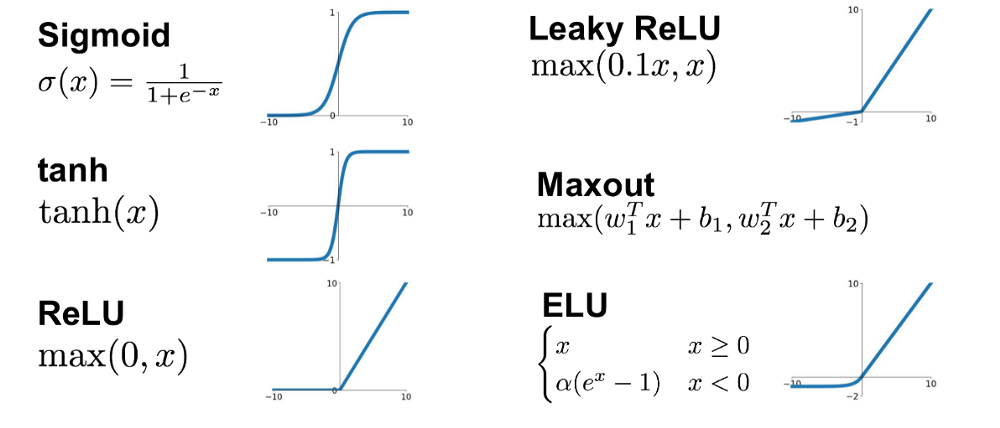
\includegraphics[width=0.80\textwidth] {./Figs/05-funcoes-ativacao.png}
                \caption{Exemplos de funções de Ativação.}\caption*{  Fonte: \cite{MCAI}} \label{fig:activation_functions}} 
            \end{figure}
            
            Em \citeonline{Almeida2013} é analisado o processo de aprendizado da rede perceptron, de forma supervisionada. Neste processo, a estrutura aprende a relacionar um conjunto observado de variáveis de entrada na rede com um ou mais valores de saída esperados denominado como valores reais ou valores verdades. Depois são avaliados os resultados do aprendizado, comparando estes valores com os valores gerados pela rede perceptron sobre o mesmo conjunto de dados, e partir desta comparação é calculada a medida de erro do treinamento.
                        
            Um critério de parada do algoritmo de treino é verificar se o erro é aceitável ou não. Caso afirmativo, a rede neural mantêm os valores dos pesos das sinapses obtidos no momento. Caso contrário, é feita uma nova época de treino tentando ajustar os pesos para obter um erro menor.
            O outro critério de parada é atingir um numero máximo permitido de épocas de treinamento. O reajuste de pesos é denominado taxa de aprendizagem.
            
            O seguinte passo no desenvolvimento de modelos de redes neurais está relacionado com a topologia que determina a quantia dos perceptrons na rede e a forma como eles se conectam, gerando redes de múltiplas camadas.        
    
        \subsection{Rede MultiLayer Perceptron (MLP)}
    
            A possibilidade de combinar duas ou mais camadas de perceptrons foi dada pela utilização de um perceptron combinador de sinal de saída. Com ele as redes neurais são ampliadas para varias colunas de perceptrons interconectados. Cada coluna é denominada uma camada oculta da rede neural. A ultima camada deve ter o número de perceptrons correspondente ao número de saídas desejadas. Na Figura \ref{fig:MLP} é apresentada  uma rede neural com 2 camadas ocultas, e cuja camada de saída possui 3 neurônios.
            
            \begin{figure}[ht]
             \center{
             	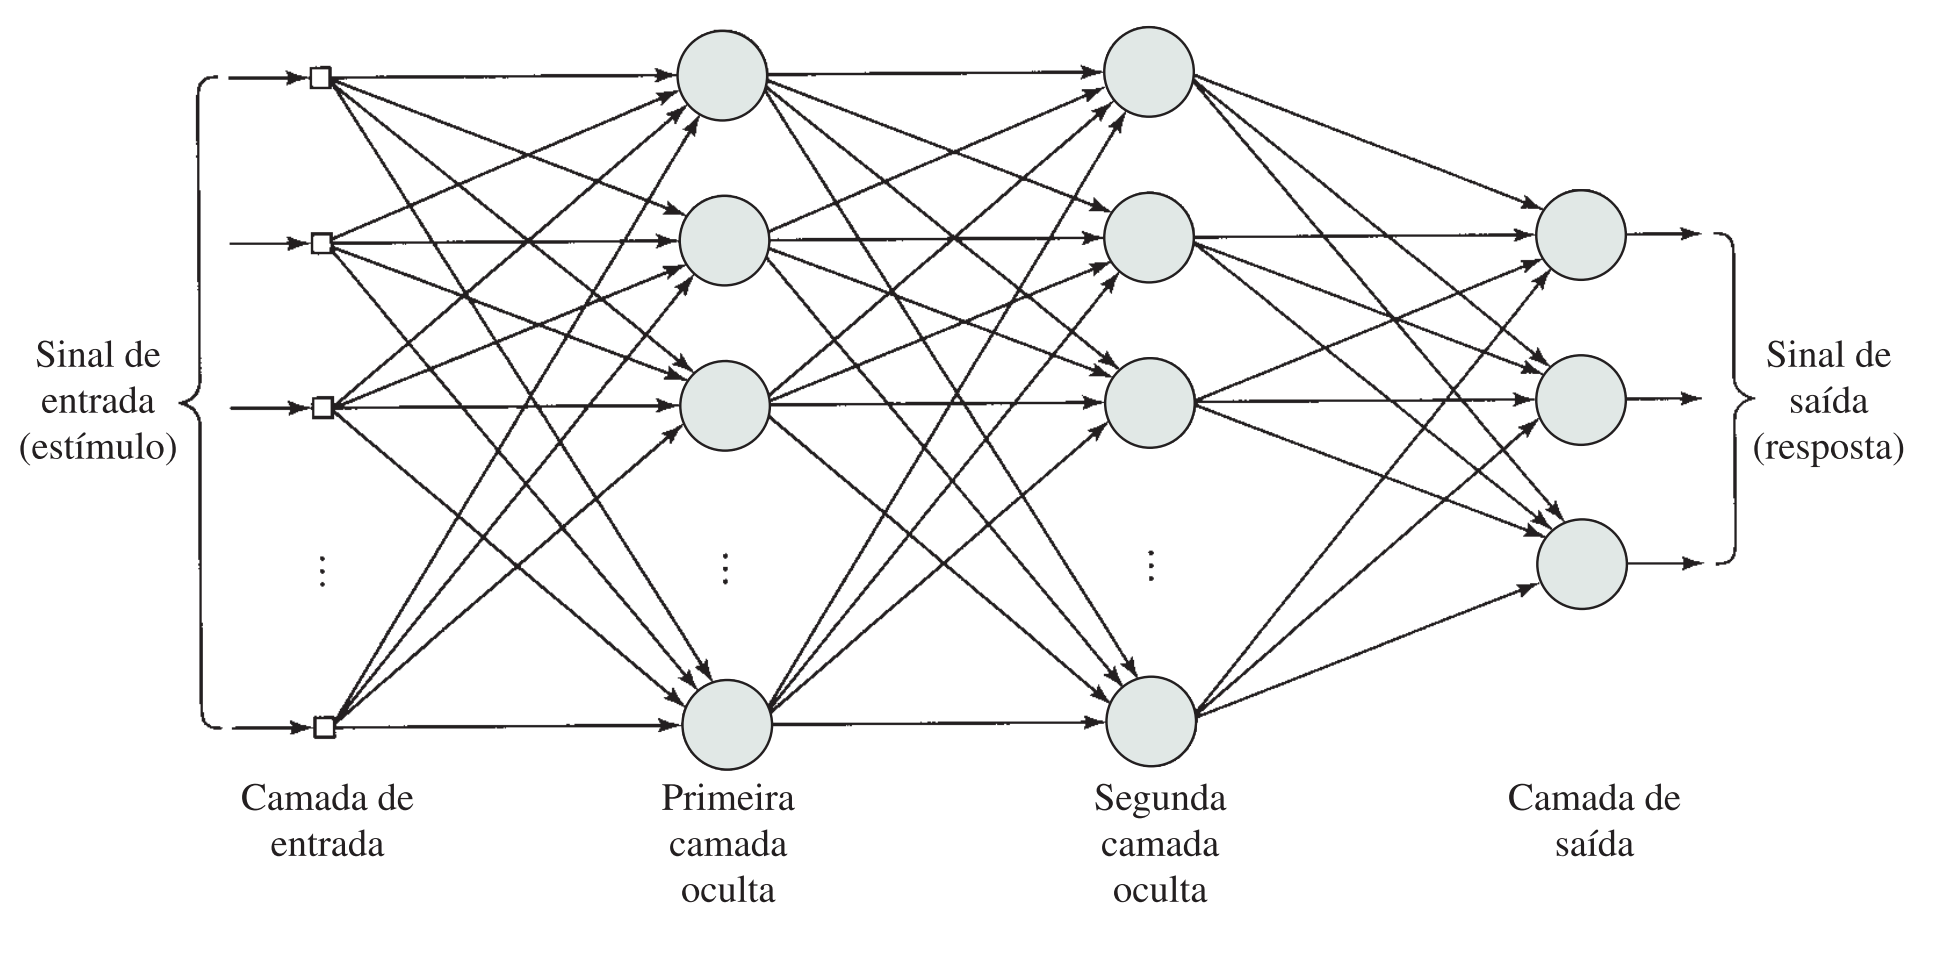
\includegraphics[width=\textwidth]
             	{./Figs/06-MLP.PNG}
             \caption{Rede de perceptrons com múltiplas camadas. }\caption*{  Fonte: \cite{Haykin1994}\label{fig:MLP}
             }}
            \end{figure}
            
            Em \citeonline{Braga2000} é postulado que através de uma camada intermediária é possível aproximar qualquer função contínua e, ainda mais, que duas camadas intermediárias são suficientes para aproximar qualquer função matemática. Se a utilização de duas ou mais camadas pode facilitar o treinamento da rede, torna-se inviável a utilização de um número grande destas, pois em cada camada oculta o erro é estimado a partir do erro na camada anterior, o que gera perda de precisão.
            
            Nas aplicações práticas, tem-se visto que em alguns casos, que a capacidade de abstração e reconhecimento de padrões das redes neurais sobrepassa as capacidades humanas. Em outros casos, uma rede pode não produzir uma resposta esperada resolvendo erroneamente um problema, assim como o cérebro humano, devido à limitações de aprendizado ou falhas nos treinos. 
              
            Para treinar de modo supervisionado uma rede MLP, o conjunto de dados de entrada deve ser dividido em em dois subconjuntos, um de \textit{treino} e um de \textit{validação}. Esses subconjuntos podem ser separados com diversas técnicas. Assim, por exemplo em \citeonline{DLB} é apresentada uma forma heurística de separação de conjuntos em ordem aleatória, com 70\% dos dados para treino e 30\% dos dados para validação.
            
            Em relação ao numero máximo de tentativas de treino permitidas, tem-se que treinos muito prolongados tendem a memorizar pesos dos valores observados nos dados de treino. Isto se traduz em perda capacidade de generalização da rede, implicando em uma dificuldade para avaliar entradas fora dos dados de treino. Esse fenômeno é conhecido como \textit{overfitting}.
            
            Existe uma outra forma de treinar uma rede MLP, chamada de validação cruzada, que foi apresentada em \cite{crossvalidation}. Essa técnica consiste em intercambiar os conjuntos de treino e de validação em diferentes épocas de treino. Nesse caso, a medida do erro de validação passa por um processo de avaliação levando em consideração o número de épocas. Avaliando o erro quadrático médio de ambos os conjuntos é possível detectar o inicio do \textit{overfitting}. Por isso, o ponto ótimo de parada do treinamento está associado ao limite inferior deste erro quadrático médio no conjunto de validação ilustrado na figura \ref{fig:validacaoCruzada} como ponto de parada antecipada ao \textit{overfitting}.
            
            \begin{figure}[ht]
              \center{
              	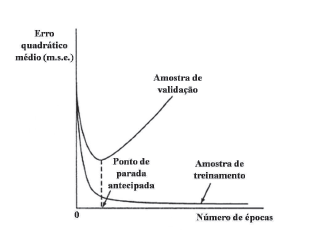
\includegraphics[width=0.5\textwidth]
              	{./Figs/07-validacaocruzada.png}
              
              \caption{Ponto ótimo de parada da validação cruzada. }\caption*{ Fonte: \cite{Haykin1994}} \label{fig:validacaoCruzada}} 
            \end{figure}
    
        \subsection{Rede perceptron Múltiplas Camadas com \textit{Backpropagation}.}
    
            O método de aprendizado para redes neurais de múltiplas camadas denominado de \textit{Backpropagation} foi apresentado em \cite{backp}, como abreviação de \textit{backward propagation of errors}, em português, retro-propagação de erros. Nesse método, o treinamento é feito em duas fases:
        
            \paragraph*{\textit{ Feed-forward} } E apresentado um vetor de entrada com vetor de saída conhecido aos neurônios da primeira camada, e calculado um vetor de saída seguindo o fluxo natural das operações na rede.
             
            \paragraph*{\textit{Feed-backward}} É calculado o gradiente do erro, para obter informação que induz decréscimo na função, dada pela direção oposta ao gradiente. Com isso, são atualizados os pesos de todas as camadas, começando pela última e seguindo o fluxo inverso da rede.
             
            Essas duas fases são esquematizadas na Figura \ref{fig: MLP2}. 
             
            \begin{figure}[ht]
             	\center{
             		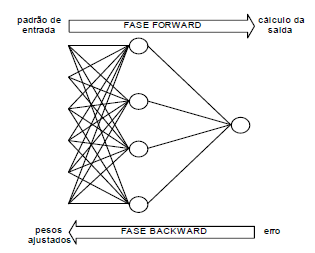
\includegraphics[width=0.65\textwidth]
             		{./Figs/08-mlp-back.png}
             	
             	\caption{Fases de treino da \textit{MLP-Back-Propagation}.}\caption*{  Fonte:  \cite{Almeida2013}}\label{fig: MLP2}}
            \end{figure}
            
            Neste método, a medida que o gradiente do erro é calculado das camadas inferiores para as superiores, sua norma  decresce com velocidade exponencial. Isto faz que nas camadas mais próximas à entrada os ajustes de pesos  sejam pequenos, tornando o aprendizado nelas  mais lento. Este problema é conhecido na literatura como \textit{vanishing gradient problem}, o problema de dissipação do gradiente.   Usualmente, os valores das taxas de aprendizagem ficam entre 0,2 e 0,8.
            
            Nos treinamentos de redes neurais MLP com \textit{backpropagation}, a validação ocorre só com a fase \textit{feedforward}, obtendo-se os erros quadráticos da camada de saída com o dado de validação observado. 
            
            Como o ponto ótimo de parada é um limite inferior, o mesmo somente é descoberto quando superado após algumas épocas de treino, dado que em procedimentos práticos a obtenção de erro é oscilatória e pelo qual é necessário manter salvos os parâmetros obtidos durante estas épocas.
            
            \paragraph{Otimizador de reajuste dos pesos} São conhecidos vários algoritmos que otimizam a convergência do reajuste dos pesos no treino de \textit{backpropagation}, como os que serão mencionados a seguir. O otimizador Momentum acelera o reajuste dos pesos em busca dos erros globais mínimos, e o RMSProp impede a busca na direção das oscilações. Um terceiro otimizador, denominado Adam pela abreviação de Adaptive Moment otimization, combina essas duas caracterpisticas. Para o algoritmo ADAM, a taxa de aprendizado pode ser arbitrada mas em \citeonline{MLM} é mencionado que uma constante com valor 0.001 tem produzido resultados positivos em problemas de predições.  
            
            Na Figura \ref{fig:otimizadores} é comparado  o comportamento de alguns otimizadores. Nesta figura é possível ver que quanto menor o custo de treinamento, maior a velocidade de convergência ao reajuste ideal dos pesos. Além disso, é visível a vantagem computacional do ADAM frente à outros otimizadores, quando se aumenta o número de iterações.
            
            \begin{figure}[ht]
            \center{
            	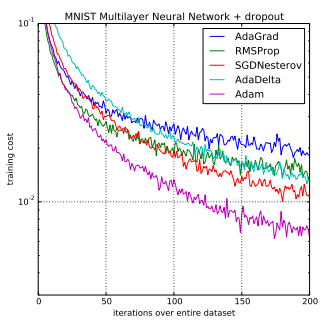
\includegraphics[width=0.70\textwidth]
            	{./Figuras/MLM/optimizers.png}
            
            \caption{Comportamento de otimizadores para MLP treinadas com \textit{Backpropagation}.}\caption*{  Fonte : \cite{MLM} }    \label{fig:otimizadores}}
        
            \end{figure}
            
    \subsection{Redes Recorrentes: O modelo GRU}\label{sec:GRU}

    As redes GRU, abreviação de \textit{Gated Recurrent Unit}, foram apresentadaspor primeira vez em \cite{gru}, sendo uma adaptação das redes LSTM (Long Short-Term Memory).
    
    As redes LSTM foram apresentadas em \cite{lstm}, e utilizam blocos de memória chamados células, que permitem que certas informações sejam mantidas na rede. A manipulação da informação é feita por portões (\textit{gates}, pelo qual o procedimento comumente é chamado \textit{gating}). Para estas redes, existem  três tipos de portões: i ) portão de esquecimento, para remover informações que já não são úteis, ii) potão de entrada, para adicionar de informações úteis ao estado da célula, e iii) portão de saída, para extrair informações úteis do estado da célula. 
    
    As redes LSTM permitiram a resolução de problemas mais complexos, porém, apresentavam ainda o problema de dissipação do gradiente, pelo qual a memoria não conseguia manter informações de sequencias longas, pelo qual era usado o termo de memória de curto prazo.
    
    As redes recorrentes GRU resolveram este problema trocando o uso do estado das células pelo uso de um estado oculto com dois novos portões. Esses portões, chamados de portão de atualização (\textit{update}) e de redefinição (\textit{reset}) decidem quais informações devem ser passadas para a saída e  podem ser treinados para manter informações de sequencias longas, sem sofrer dissipação dos valores. 
    
    Em \cite{DLB}, esses portões são citados como as estruturas úteis para solucionar problemas de predições. Na Figura \ref{fig:gru-arch} são apresentados dois modelos de redes, um  LSTM e um GRU, indicando os portões em cada um delas. 
         	
    \begin{figure}[ht]
    	\center{
    		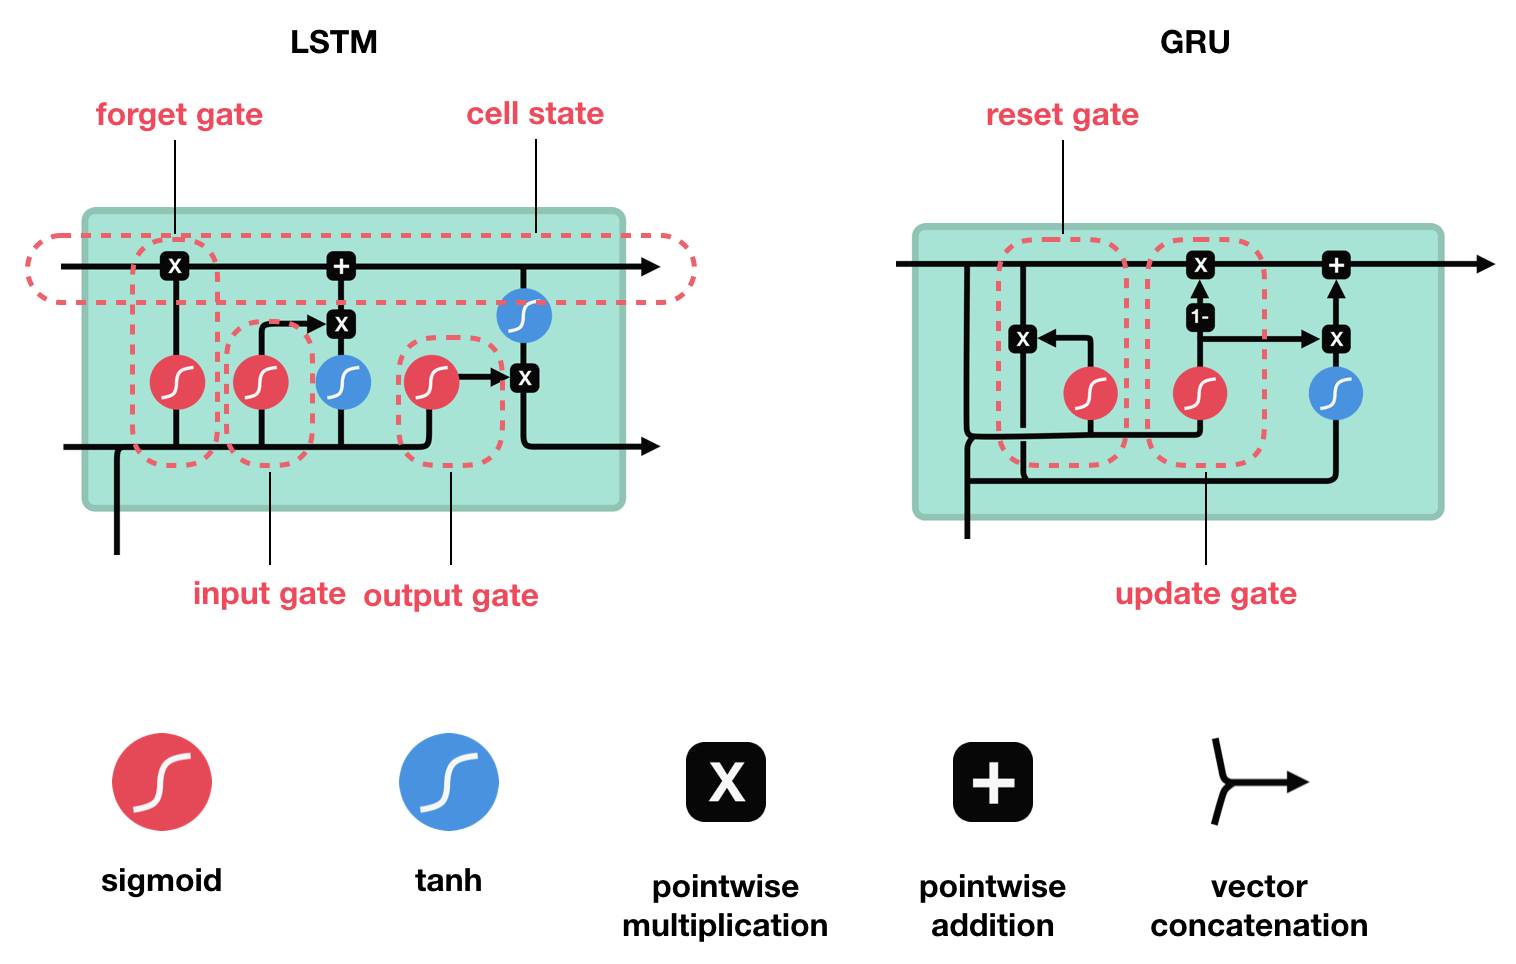
\includegraphics[width=0.80\textwidth]
    		{./Figs/10-portoes-rnns.png}
    	 	\caption{Arquitetura do modelo GRU.}\caption*{  Fonte: \cite{DLB}} \label{fig:gru-arch}}
    \end{figure}
    
    As redes GRU permitiram então a resolução de problemas com sequencias longas de dados, resolvendo o problema de memória a curto prazo. Então a maior dificuldade que poderia surgir ainda nos treinamentos supervisionados teria a ver com o overfitting, pelo qual foi proposta mais uma ferramenta para evitar que a rede memoriza-se além do desejado: o método \textit{dropout}.
    
    \subsubsection{Dropout} \label{sec:drop_fund}
    
    O método de \textit{Dropout} foi apresentado em \cite{dropout}, termo traduzido ao português na literatura como abandono, e propõe a remoção temporária de alguma célula da rede. 
    
    Em \cite{dropoutapp} foi aplicado \textit{dropout} no treino de uma rede neural, no qual, em cada época de treinamento são desligadas aleatoriamente algumas células da camada de entrada e algumas outras das camadas ocultas, sendo todas ligadas novamente no final da época. Com isso, em cada época do treino apenas uma amostra dos dados é processada por um subconjunto das células ocultas.  
    
    Esta técnica procura que a aleatoriedade da escolha de células em cada época induza uma redução na dependência entre elas as células no processo de ajuste, fazendo que cada unidade gere padrões que não dependam dos aprendidos pelas outras. No momento do teste, todos os pesos são multiplicados pela probabilidade da sua célula ter sido desligada. 
    
    Em \cite{dropoutapp} são obtidos bons resultados no treino da rede com \textit{dropout} quando, em cada época,  são desligadas 50\% das células em camadas ocultas e 20\% das células na camada de entrada.
    

    

